\chapter{Hardware implementeringen og operativ system}\label{kap:hardware}

I dette kapitel vil den komplette software og hardware løsning blive gennemgået som gør det muligt at udfører den digitale behandling af lydsignalet.
\husk{JJ}{Kort beskrivelse af de mellemliggende trin}
Til sidst vil der være en gennemgang af de nærliggende forbedringer og optimeringer.


\begin{enumerate}
	\item Overblik af OS, lagdelt model
	\item Beskrivelse af Hardware lag - beskrivelse af de forskellige setups og hvorfor - fordele og ulæmper.
	\begin{enumerate}
		\item Initalisering af systemet som helhed - fastsættelse af beregningspunkter.
		\item Fastsættelse af clockfrekvens
		\item ADC (simon)
		\item LCD Driver (søren)
		\item UART
		\item DAC / SPI
	\end{enumerate}
	\item håndtering af indgående lyssignal i de forskellige modes
	\item FPU math
	\item Schedulering af taskt - task model 
	\item Beskrivelse af de enkelte tasks
	\item Shell (ANSI / VT100)
	\item Quealizer profile model
	\item Debugging og task time profiling
	
\end{enumerate}

\section{Det vigtigste er lyden}
Den absolut primære funktion af equalizeren   


\husk{JJ}{sektion der beskriver indledende hvordan tilgangen til design af OS har været med baggrund i krav om sampling og gengivelse i realtime}

\section{Operativ systemet}

\begin{figure}[h!]
	\centering
	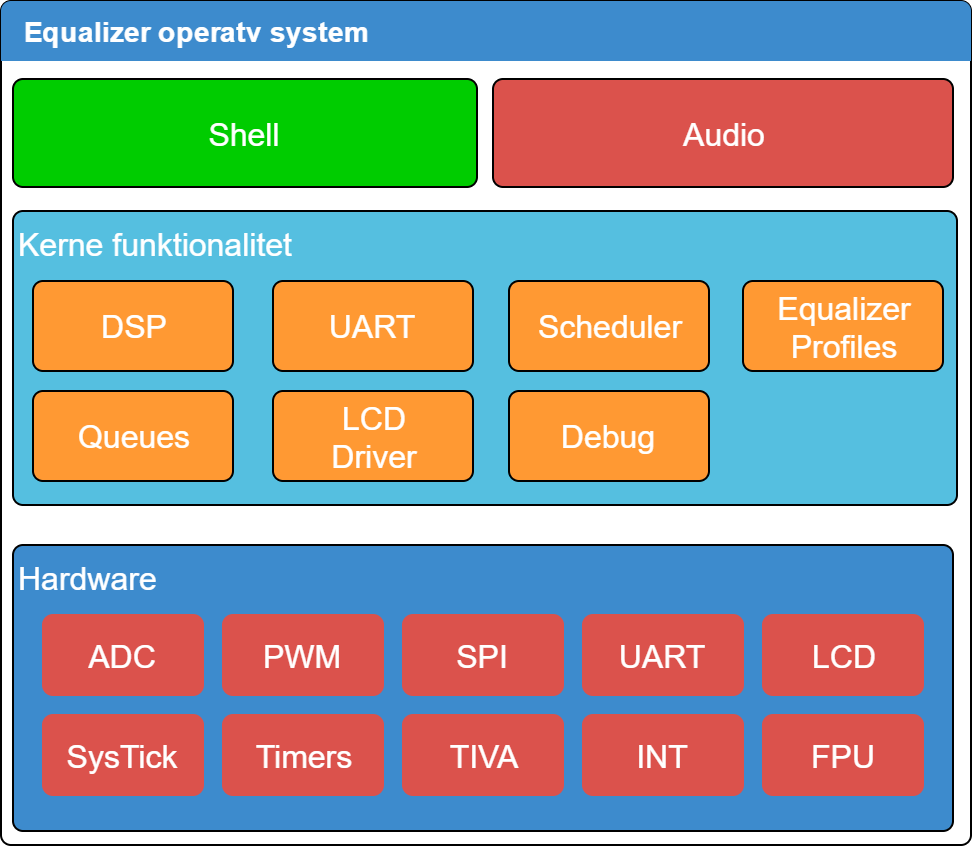
\includegraphics[width=.8\textwidth]{billeder/eq_os.png}
	\caption{Arkitektur af equalizerens operativ system.}
	\label{fig:eq_os}
\end{figure}
\FloatBlock


\section{Schedulering}




\section{Hardware lag}


\section{Equalizer modul og profiler}

\section{Shell}

\section{Debugging, process timing og mulige udfordringer}

\section{Pin mapping}

\husk{JJ}{Oversæt excel ark til \LaTeX}
\husk{JJ}{Dettte skema skal overflyttes som bilag}

\section{Udvidelser}

\begin{enumerate}
	\item I2C intraface
	\item Flash lager
	\item Flere shell commmandoer
\end{enumerate}
